%%%%%%%%%%%%%%%%%%%%%%%%%%%%%%%%%%%%%%%%%
% Beamer Presentation
% LaTeX Template
% Version 2.0 (March 8, 2022)
%
% This template originates from:
% https://www.LaTeXTemplates.com
%
% Author:
% Vel (vel@latextemplates.com)
%
% License:
% CC BY-NC-SA 4.0 (https://creativecommons.org/licenses/by-nc-sa/4.0/)
%
%%%%%%%%%%%%%%%%%%%%%%%%%%%%%%%%%%%%%%%%%

%%%%%%%%%%%%%%%%%%%%%%%%%%%%%%%%%%%%%%%%%
% This presentation template is an adaptation of the template mentioned above. It has been created by Giovanni Spadaro and it is available on GitHub (https://github.com/Giovo17/presentation-template-unict-lm-data).
%%%%%%%%%%%%%%%%%%%%%%%%%%%%%%%%%%%%%%%%%

%----------------------------------------------------------------------------------------
%	PACKAGES AND OTHER DOCUMENT CONFIGURATIONS
%----------------------------------------------------------------------------------------

\documentclass[
	11pt, % Set the default font size, options include: 8pt, 9pt, 10pt, 11pt, 12pt, 14pt, 17pt, 20pt
	%t, % Uncomment to vertically align all slide content to the top of the slide, rather than the default centered
	%aspectratio=169, % Uncomment to set the aspect ratio to a 16:9 ratio which matches the aspect ratio of 1080p and 4K screens and projectors
]{beamer}

\graphicspath{{img/}} % Specifies where to look for included images (trailing slash required)

\usepackage{booktabs} % Allows the use of \toprule, \midrule and \bottomrule for better rules in tables

%----------------------------------------------------------------------------------------
%	SELECT LAYOUT THEME
%----------------------------------------------------------------------------------------

% Beamer comes with a number of default layout themes which change the colors and layouts of slides. Below is a list of all themes available, uncomment each in turn to see what they look like.

%\usetheme{default}
%\usetheme{AnnArbor}
%\usetheme{Antibes}
%\usetheme{Bergen}
%\usetheme{Berkeley}
%\usetheme{Berlin}
\usetheme{Boadilla}
%\usetheme{CambridgeUS}
%\usetheme{Copenhagen}
%\usetheme{Darmstadt}
%\usetheme{Dresden}
%\usetheme{Frankfurt}
%\usetheme{Goettingen}
%\usetheme{Hannover}
%\usetheme{Ilmenau}
%\usetheme{JuanLesPins}
%\usetheme{Luebeck}
%\usetheme{Madrid}
%\usetheme{Malmoe}
%\usetheme{Marburg}
%\usetheme{Montpellier}
%\usetheme{PaloAlto}
%\usetheme{Pittsburgh}
%\usetheme{Rochester}
%\usetheme{Singapore}
%\usetheme{Szeged}
%\usetheme{Warsaw}

%----------------------------------------------------------------------------------------
%	SELECT COLOR THEME
%----------------------------------------------------------------------------------------

% Beamer comes with a number of color themes that can be applied to any layout theme to change its colors. Uncomment each of these in turn to see how they change the colors of your selected layout theme.

%\usecolortheme{albatross}
%\usecolortheme{beaver}   % red
%\usecolortheme{beetle}
%\usecolortheme{crane}   % yellow
%\usecolortheme{dolphin}  % purple
%\usecolortheme{dove}   % white
%\usecolortheme{fly}   % grey
%\usecolortheme{lily}   % purple
%\usecolortheme{monarca}   % yellow background and black
%\usecolortheme{seagull}
%\usecolortheme{seahorse}
%\usecolortheme{spruce}   % green
\usecolortheme{whale}
%\usecolortheme{wolverine}

%----------------------------------------------------------------------------------------
%	SELECT FONT THEME & FONTS
%----------------------------------------------------------------------------------------

% Beamer comes with several font themes to easily change the fonts used in various parts of the presentation. Review the comments beside each one to decide if you would like to use it. Note that additional options can be specified for several of these font themes, consult the beamer documentation for more information.

\usefonttheme{default} % Typeset using the default sans serif font
%\usefonttheme{serif} % Typeset using the default serif font (make sure a sans font isn't being set as the default font if you use this option!)
%\usefonttheme{structurebold} % Typeset important structure text (titles, headlines, footlines, sidebar, etc) in bold
%\usefonttheme{structureitalicserif} % Typeset important structure text (titles, headlines, footlines, sidebar, etc) in italic serif
%\usefonttheme{structuresmallcapsserif} % Typeset important structure text (titles, headlines, footlines, sidebar, etc) in small caps serif

%------------------------------------------------

%\usepackage{mathptmx} % Use the Times font for serif text
\usepackage{palatino} % Use the Palatino font for serif text

%\usepackage{helvet} % Use the Helvetica font for sans serif text
\usepackage[default]{opensans} % Use the Open Sans font for sans serif text
%\usepackage[default]{FiraSans} % Use the Fira Sans font for sans serif text
%\usepackage[default]{lato} % Use the Lato font for sans serif text

%----------------------------------------------------------------------------------------
%	SELECT INNER THEME
%----------------------------------------------------------------------------------------

% Inner themes change the styling of internal slide elements, for example: bullet points, blocks, bibliography entries, title pages, theorems, etc. Uncomment each theme in turn to see what changes it makes to your presentation.

%\useinnertheme{default}
\useinnertheme{circles}
%\useinnertheme{rectangles}
%\useinnertheme{rounded}
%\useinnertheme{inmargin}

%----------------------------------------------------------------------------------------
%	SELECT OUTER THEME
%----------------------------------------------------------------------------------------

% Outer themes change the overall layout of slides, such as: header and footer lines, sidebars and slide titles. Uncomment each theme in turn to see what changes it makes to your presentation.

%\useoutertheme{default}
%\useoutertheme{infolines}
\useoutertheme{miniframes}
%\useoutertheme{smoothbars}
%\useoutertheme{sidebar}
%\useoutertheme{split}
%\useoutertheme{shadow}
%\useoutertheme{tree}
%\useoutertheme{smoothtree}

%\setbeamertemplate{footline} % Uncomment this line to remove the footer line in all slides
%\setbeamertemplate{footline}[page number] % Uncomment this line to replace the footer line in all slides with a simple slide count

%\setbeamertemplate{navigation symbols}{} % Uncomment this line to remove the navigation symbols from the bottom of all slides

%----------------------------------------------------------------------------------------
%	PRESENTATION INFORMATION
%----------------------------------------------------------------------------------------

\title[Final report]{Three Phase Multi-Level Inverter Topologies and Modulation Techniques} % The short title in the optional parameter appears at the bottom of every slide, the full title in the main parameter is only on the title page

%\subtitle{Optional Subtitle} % Presentation subtitle, remove this command if a subtitle isn't required

\author[Huan Nguyen-Duy]{Huan Nguyen-Duy \\ Student ID: 2390703} % Presenter name(s), the optional parameter can contain a shortened version to appear on the bottom of every slide, while the main parameter will appear on the title slide

\institute[HCMUTE]{Ho Chi Minh City University of Technology and Education} % Your institution, the optional parameter can be used for the institution shorthand and will appear on the bottom of every slide after author names, while the required parameter is used on the title slide and can include your email address or additional information on separate lines

\date[Apr/08/2024]{} % Presentation date or conference/meeting name, the optional parameter can contain a shortened version to appear on the bottom of every slide, while the required parameter value is output to the title slide

%----------------------------------------------------------------------------------------

\begin{document}

%----------------------------------------------------------------------------------------
%	TITLE SLIDE
%----------------------------------------------------------------------------------------

\begin{frame}
    \begin{figure}
		
\includegraphics[width=0.4\linewidth]{HCMUTE.png}
	\end{figure}
	\titlepage
\end{frame}

%----------------------------------------------------------------------------------------
%	TABLE OF CONTENTS SLIDE
%----------------------------------------------------------------------------------------

% The table of contents outputs the sections and subsections that appear in your presentation, specified with the standard \section and \subsection commands. You may either display all sections and subsections on one slide with \tableofcontents, or display each section at a time on subsequent slides with \tableofcontents[pausesections]. The latter is useful if you want to step through each section and mention what you will discuss.

\begin{frame}
	\frametitle{Table of Contents} % Slide title, remove this command for no title

	\begin{columns}
		\begin{column}{0.5\textwidth}
			\tableofcontents % Output the table of contents (all sections on one slide)
		\end{column}
		\begin{column}{0.5\textwidth}
            \centering
            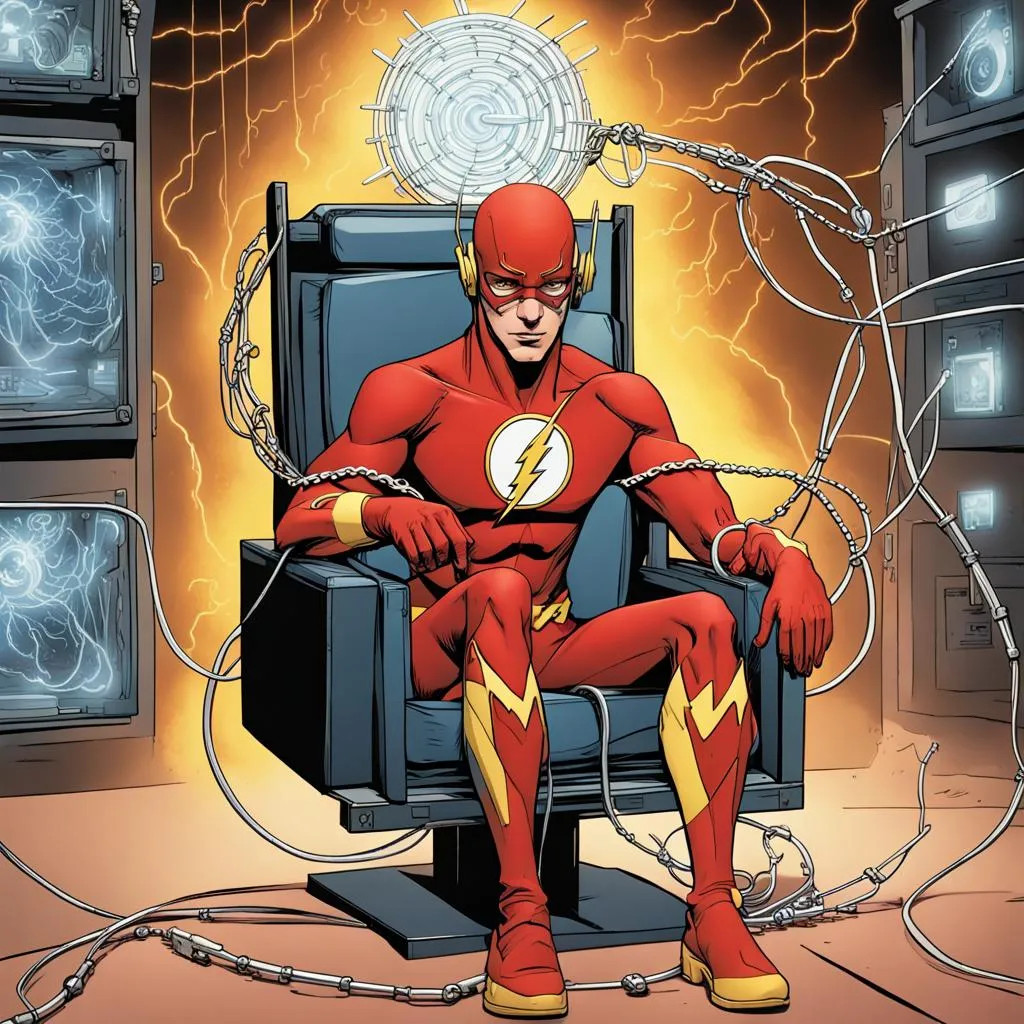
\includegraphics[width=\linewidth]{table.jpg}
        \end{column}
	\end{columns}
	
\end{frame}

%----------------------------------------------------------------------------------------
%	Overview Slides
%----------------------------------------------------------------------------------------

\section{Overview}
\begin{frame}{Abstract}
	\begin{itemize}
		\footnotesize
		\item{To mention the vital role of power electronic converter in the power production domain}
		\item{The paper reveiews methodologies to control \textbf{three-phase multi-level Inverter} by PWD control techniques}    
		\item{Proposal \textbf{three-phase multi-level Inverter topologies} and \textbf{Modulation Techniques}}
		\item{comparison among PWM control techniques \textbf{phase disposition (PD)}, 
				\textbf{phase opposite disposition (POD)}, and \textbf{alternate phase opposite disposition (APOD)}}
		\item{Analysing \textbf{THD} and \textbf{common mode} between methodologies}
	\end{itemize}
\end{frame}


\begin{frame}{Reference Papers}
	\begin{itemize}
		\footnotesize
		\item{Anup Kumar Panda and Yellasiri Suresh, “Research on cascaded
		multilevel inverter with single DC source by using three-phase
		transformers,” Electrical Power and Energy Systems. no 40, pp. 9–20,
		2012.}
		\item{Bendre A, Krstic S, Meer JV and Venkataramanan G., “Comparative
		evaluation of modulation algorithms for neutral point clamped
		converters,” IEEE Trans Ind Appl 2005;41:634–43.}
		\item{  Colak I, Kabalci E and Bayindir R., “Review of multilevel voltage
		source inverter topologies and control schemes,” Energy Convers
		Manag 2011; 52:1114–28.}
		\item{  Anup Kumar Panda.: Yellasiri Suresh.: Research on cascaded
		multilevel inverter with single DC source by using three-phase
		transformers. Electrical Power and Energy Systems. no 40, pp. 9–20,
		2012.} 
		\item{Suresh.Y., Panda A.K.: Research on a cascaded multilevel inverter by
		employing three-phase transformers. IET Power Electron., Vol. 5, no.
		5, pp. 561–570, 2012}
		\item{R. Gonzalez, E. Gubia, J. Lopez, and L. Marroyo, “Transformer less
		single phase multilevel-based photovoltaic inverter,” IEEE Trans. Ind.
		Electron., vol. 55, no. 7, pp. 2694–2702, Jul. 2008}
	\end{itemize}
\end{frame}

\begin{frame}{Review Objective}
	\begin{itemize}
		\setlength{\itemsep}{10pt}
		\footnotesize
		\item {Three-Phase multi-level Inverter}
		\begin{itemize}
			\setlength{\itemsep}{10pt}
			\footnotesize
			\item{Diode clamped Inverter}
			\item{Flyting capacitor Inverter}
			\item{Cascaded H-Bridge Inverter}
		\end{itemize}
		\item{Single DC source with single phase transformer H-Bridge (topology 1)}
		\item{Single DC source with single phase transformer H-Bridge (topology 2)}
		\item{Modulation techniques}
		\begin{itemize}
			\setlength{\itemsep}{10pt}
			\footnotesize
			\item {phase disposition (PD)}
			\item {phase opposite disposition (POD)}
			\item {alternate phase opposite disposition (APOD)}
		\end{itemize}
	\end{itemize}
\end{frame}


%----------------------------------------------------------------------------------------
%	Introduction Slides
%----------------------------------------------------------------------------------------

\section{Introduction}
\begin{frame}{Introduction about three-Phase Inverter}
	\begin{figure}
		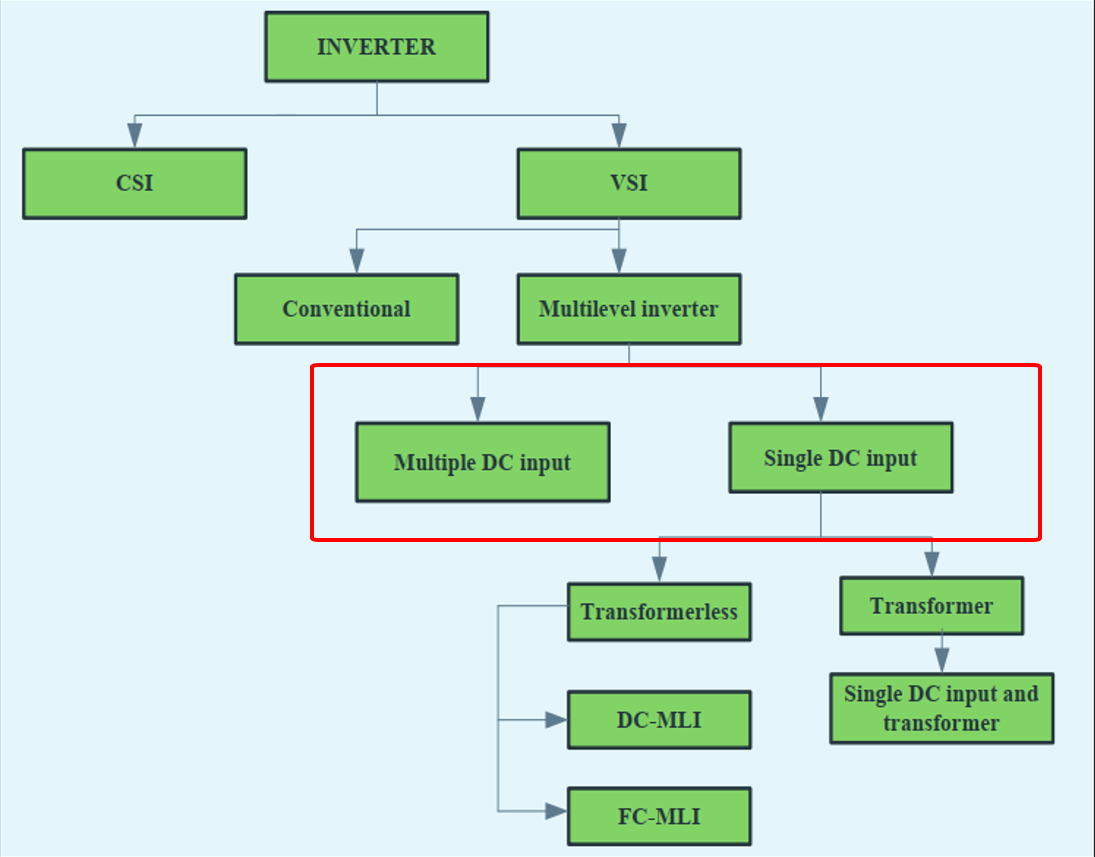
\includegraphics[width=0.7\linewidth]{introthreephaseinverter.png}
	\end{figure}
\end{frame}

\begin{frame}{Introduction about three-Phase Inverter}
	\begin{itemize}
		\setlength{\itemsep}{10pt}
		\item {The three-phase converter include voltage source Inverter (VSI) and current source Inverter (CSI)}
		\item {voltage source Inverter (VSI)}
		\begin{itemize}
			\setlength{\itemsep}{10pt}
			\item {fundamental three-phase Inverter with 2 level}
			\item {multi-level three-phase Inverter (3, 5, or 7 level)}
		\end{itemize}
	\end{itemize}
\end{frame}

\begin{frame}{Three-Phase multi-level Inverter with Diode clamped Inverter}
	\begin{figure}
		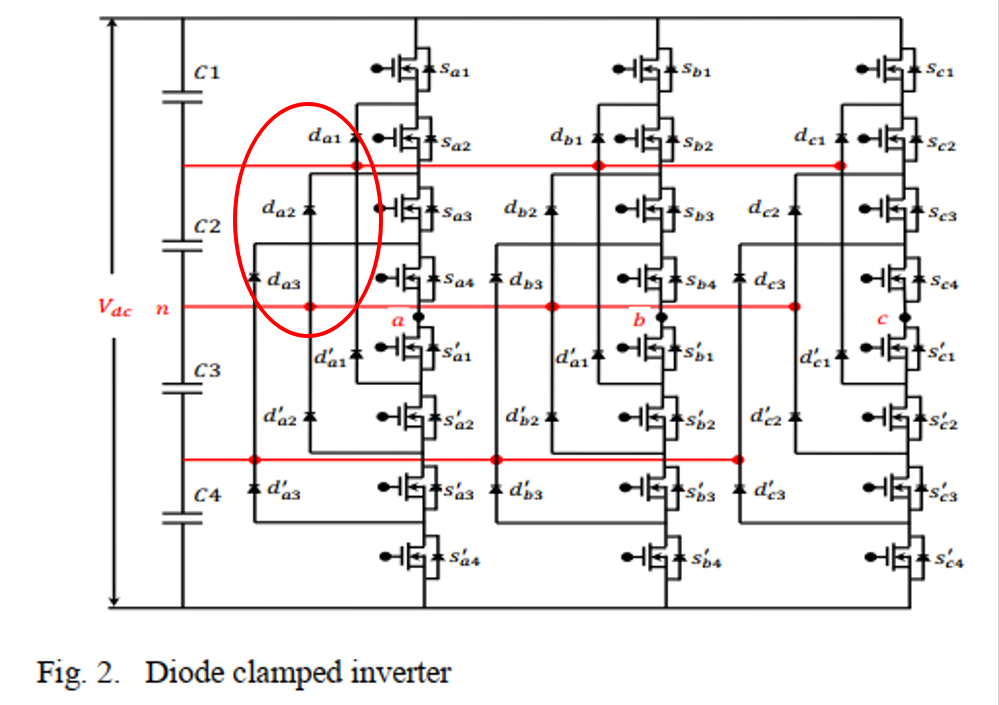
\includegraphics[width=0.7\linewidth]{diodeClamped.png}
	\end{figure}
\end{frame}

\begin{frame}{Three-Phase multi-level Inverter with Diode clamped Inverter}
	\begin{itemize}
		\setlength{\itemsep}{10pt}
		\item {three phase multi-level 5 steps using diode clamped Inverter}
		\item {Using single source DC and containing DC bus voltage with 4 capacitor C1, C2, C3, and C4}
		\item {Each capacitor have one supply voltage and single capacitor voltage is limited by the voltage stress from switches}
		\item {using cascaded diodes to connect from switches S' to S}
	\end{itemize}
\end{frame}

\begin{frame}{Three-Phase multi-level Inverter with Flyting capacitor Inverter}
	\begin{figure}
		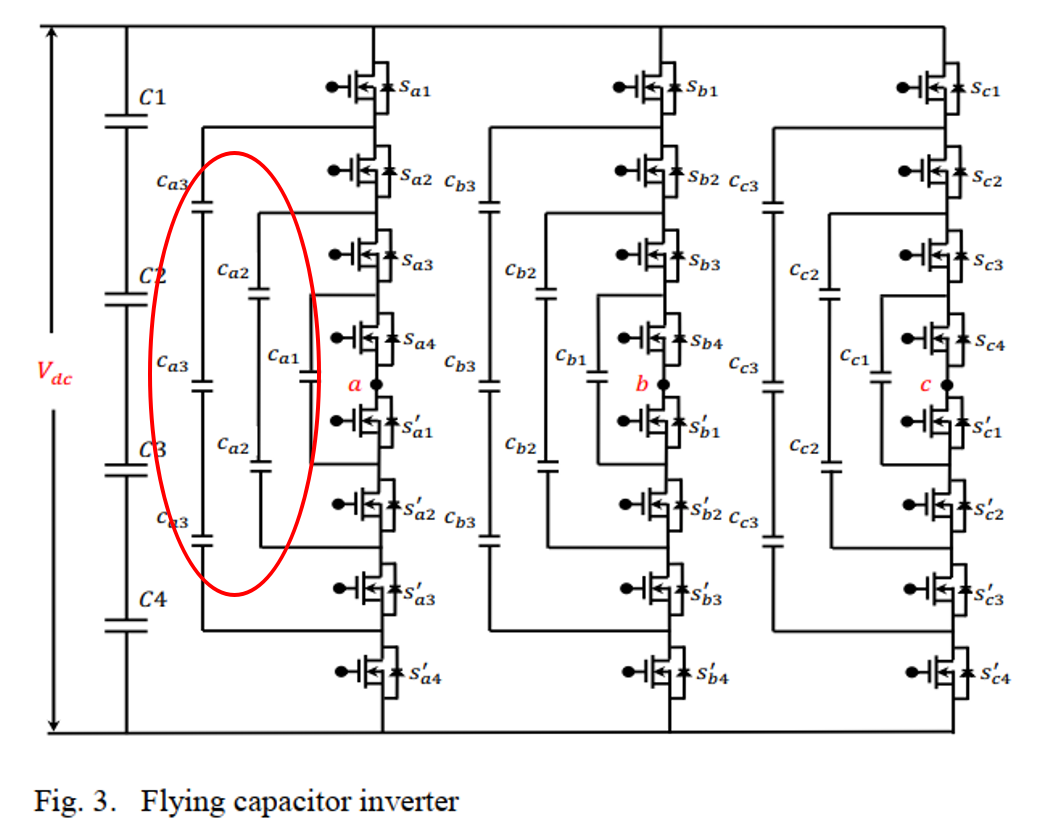
\includegraphics[width=0.6\linewidth]{flyingcap.png}
	\end{figure}
\end{frame}

\begin{frame}{Three-Phase multi-level Inverter with Flyting capacitor Inverter}
	\begin{itemize}
		\setlength{\itemsep}{10pt}
		\item {three phase multi-level 5 steps using Flyting capacitor Inverter}
		\item {Using single source DC and containing DC bus voltage with 4 capacitor C1, C2, C3, and C4}
		\item {Each capacitor have one supply voltage and single capacitor voltage is limited by the voltage stress from switches}
		\item {using cascaded capacitor to connect from switches S' to S}
	\end{itemize}
\end{frame}

\begin{frame}{Multiple DC sources with H-Bridge Inverter}
	\begin{figure}
		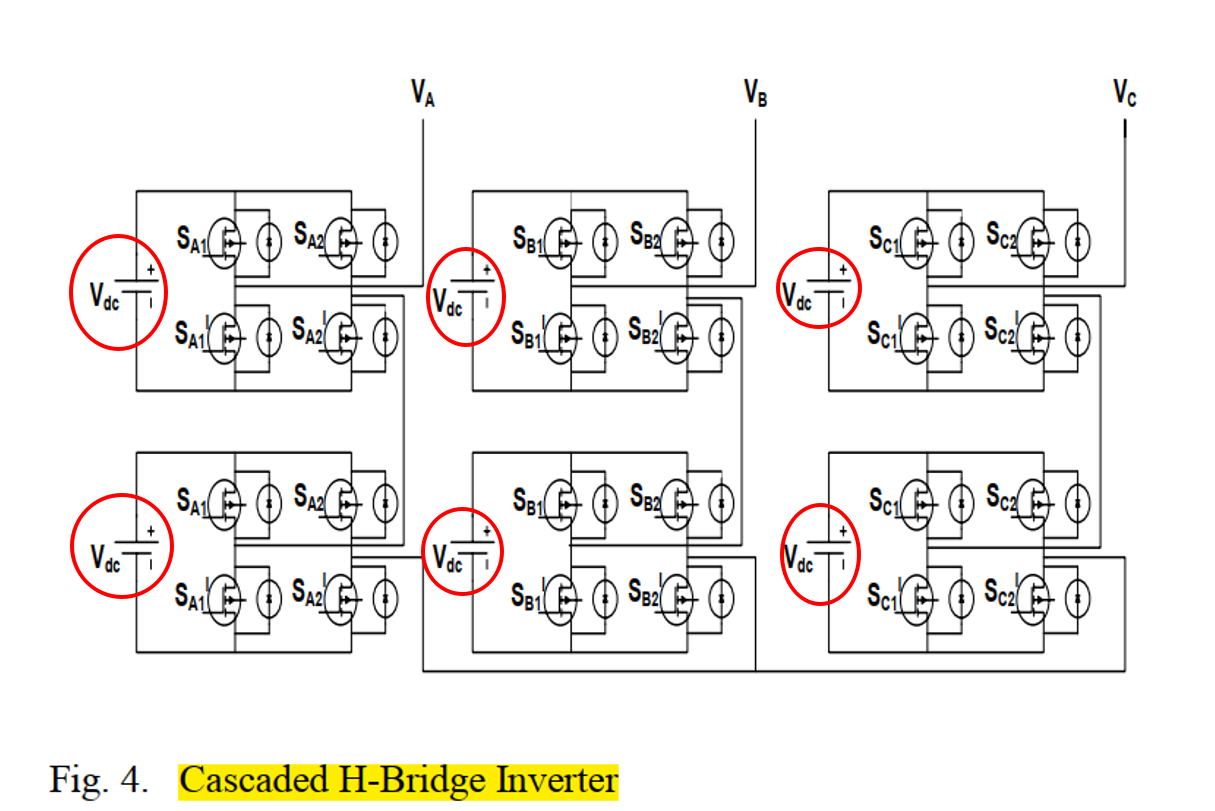
\includegraphics[width=0.7\linewidth]{cascade_Hbridge.png}
	\end{figure}
\end{frame}

\begin{frame}{Multiple DC sources with H-Bridge Inverter}
	\begin{itemize}
		\setlength{\itemsep}{10pt}
		\item {Using Multiple DC source for each full-Bridge Inverters}
		\item {containing 6 full-Bridge Inverters that divide to three level}
		\item {The cascaded level 1, 2, and 3 corresponding with phase A, B, and C respectively}
		\item {The drawback of Multi-DC source H-Bridge Inverter is using a lot of DC source}
	\end{itemize}
\end{frame}

\begin{frame}{Single DC source with single phase transformer H-Bridge (topology 1)}
	\begin{figure}
		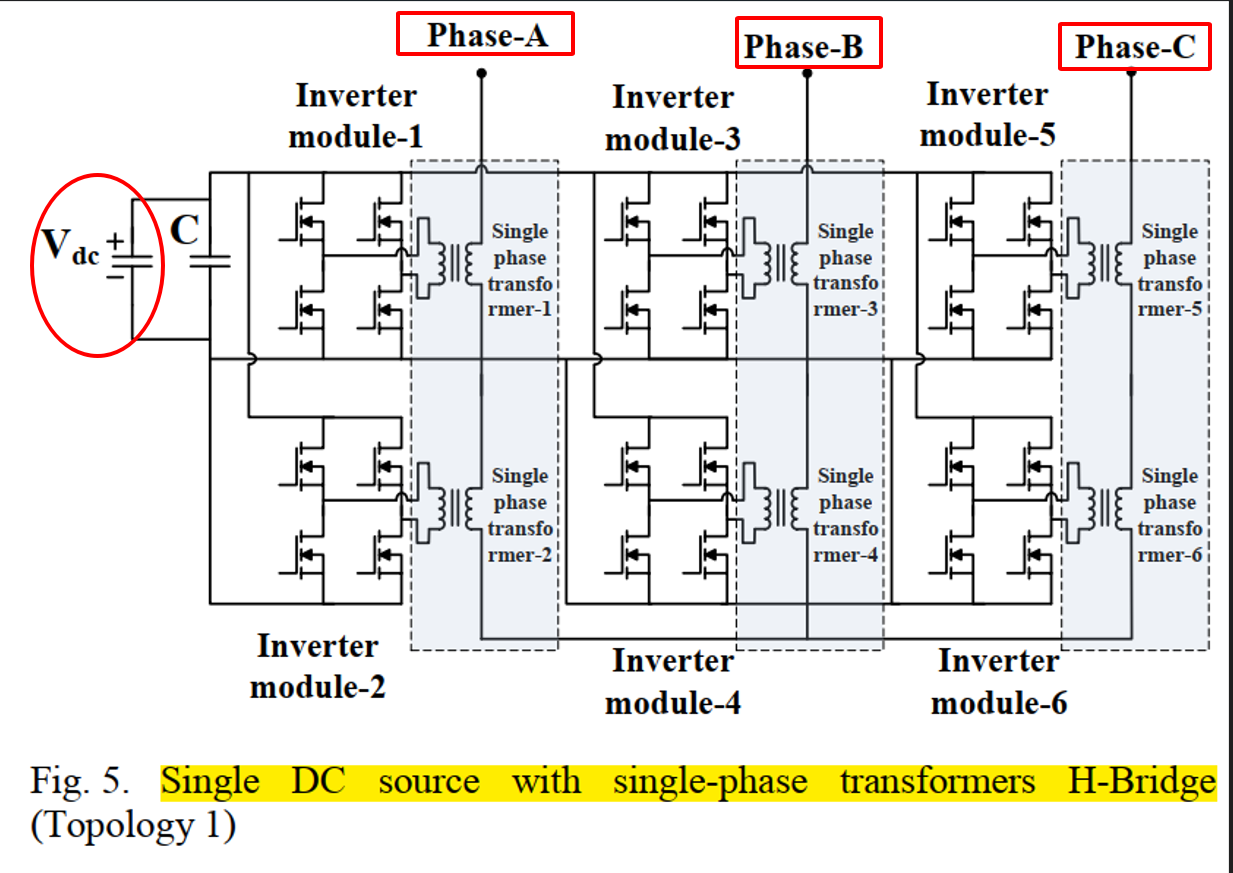
\includegraphics[width=0.7\linewidth]{Topology1.png}
	\end{figure}
\end{frame}

\begin{frame}{Single DC source with single phase transformer H-Bridge (topology 1)}
	\begin{itemize}
		\setlength{\itemsep}{10pt}
		\item {Using only one DC source for a System}
		\item {transformers are imported between levels to gain amplification of output signal}
		\item {The cascaded level 1, 2, and 3 corresponding with phase A, B, and C respectively}
		\item {the benefit of this System is using only a single DC source}
	\end{itemize}
\end{frame}


\begin{frame}{Single DC source with single phase transformer H-Bridge (topology 2)}
	\begin{figure}
		\includegraphics[width=0.6\linewidth]{Topology2.png}
	\end{figure}
\end{frame}

\begin{frame}{Single DC source with single phase transformer H-Bridge (topology 2)}
	\begin{itemize}
		\setlength{\itemsep}{8pt}
		\item {Using only one DC source for a System}
		\item {transformers are imported between levels to gain amplification of output signal}
		\item {The cascaded level 1, 2, and 3 corresponding with phase A, B, and C respectively}
		\item {Three phase transformer 2 (below) is connected directly to LOAD}
		\item {in terms of increasing voltage level by connecting the second terminal of the transformer 2 to ouput LOAD
		that is the advantage of topology 2 comparing with topology 1}
	\end{itemize}
\end{frame}

\begin{frame}{Modulation techniques}
    \begin{figure}
        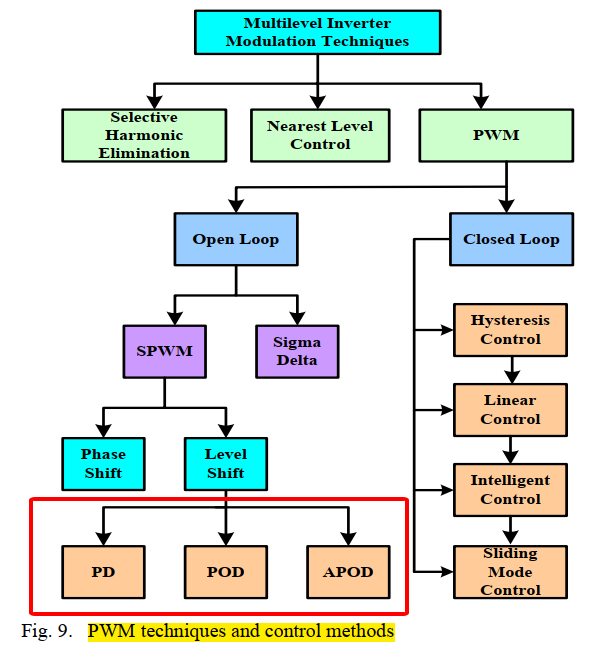
\includegraphics[width=0.45\linewidth]{PWD.png}
    \end{figure}
\end{frame}

\begin{frame}{Modulation techniques}
    \begin{itemize}
		\item {We forcus on three methods using PWD control level shift}
		\begin{itemize}
			\setlength{\itemsep}{10pt}
			\item {\textbf{PD:} this method reduces dramatically THD of the three-phase multi-level Inverter. However, the drawback of this method increases common mode.}
			\item {\textbf{POD and APOD:} By the Contrast, both methodologies will increase THD and reduce the common mode}
		\end{itemize}
	\end{itemize}
\end{frame}





%----------------------------------------------------------------------------------------
%	Content Slides
%----------------------------------------------------------------------------------------

\section{Content}
\begin{frame}{Diode clamped Inverter}
	
\end{frame}


%----------------------------------------------------------------------------------------
%	Result Slides
%----------------------------------------------------------------------------------------

\section{Result}
\begin{frame}{Content}
	
\end{frame}

%----------------------------------------------------------------------------------------
%	Result Slides
%----------------------------------------------------------------------------------------

\section{Conclusion}
\begin{frame}{Content}
	
\end{frame}


%----------------------------------------------------------------------------------------
%	PRESENTATION BODY SLIDES
%----------------------------------------------------------------------------------------


\include{sections/section1}
\include{sections/section2}
\include{sections/section3}
\include{sections/section4}


%----------------------------------------------------------------------------------------
%	CLOSING SLIDE
%----------------------------------------------------------------------------------------

\begin{frame}[plain] % The optional argument 'plain' hides the headline and footline
	\begin{center}
		{\Huge \textbf{Thanks for your attention}} \\
		\vspace{30px}
		{\textbf{Presentation: Huan Nguyen-Duy}}
            
	\end{center}
\end{frame}

%----------------------------------------------------------------------------------------

\end{document} 